\section{Analoge und Digitale Signale}

\begin{defi}{Digitales Signal}
    Ein digitales Signal ist eine spezielle Form eines Signals, welches:
    \begin{itemize}
        \item einen abgegrenzten und gestuften Wertvorrat umfasst
        \item in der zeitlichen Abfolge nur tz bestimmten periodischen Zeitpunkten definiert ist bzw. eine Veränderung im Signalwert aufweist.
    \end{itemize}

    z. B. TTL-Logikpegel mit \texttt{HIGH} (2.7 bist 5V) und \texttt{LOW} (0 bis 0.5V)
\end{defi}

\begin{defi}{Analoge Signale}
    Analoge Signale sind im Gegensatz zu digitalen Signalen sowohl im Wertebereich als auch zeitlichem Verlauf kontinuierlich.

    Ein Analogsignal ist eine Form eines Signals mit stufenlosem und unterbrechungsfreiem Verlauf.
    Ein Analogsignal wird als glatte Funktion beschrieben und es lässt sich damit beispielsweise der zeitlich kontinuierlichen Verlauf einer physikalischen Größe beschreiben.

    Viele Sensoren geben z. B. ein analoges Signal zurück, wenn sie veränderbare Widerstände nutzen (Licht-empfindlich, Temperatur-empfindlich etc.).
\end{defi}

\begin{defi}{Digitalisierung}
    Die Umwandlung eines analogen Signals in ein digitales Signal nennt man \emph{Digitalisierung}.
\end{defi}

\begin{bonus}{Abtastung}
    Analoge Signale werden regelmäßig gemessen.

    Dabei wird der Wert zu dem n-ten Zeitpunkten $t_n = n \cdot \Delta t$ gemessen.

    Bei dem \texttt{Hold}-Verfahren wird der letzte gemessene Wert gehalten:

    \begin{center}
        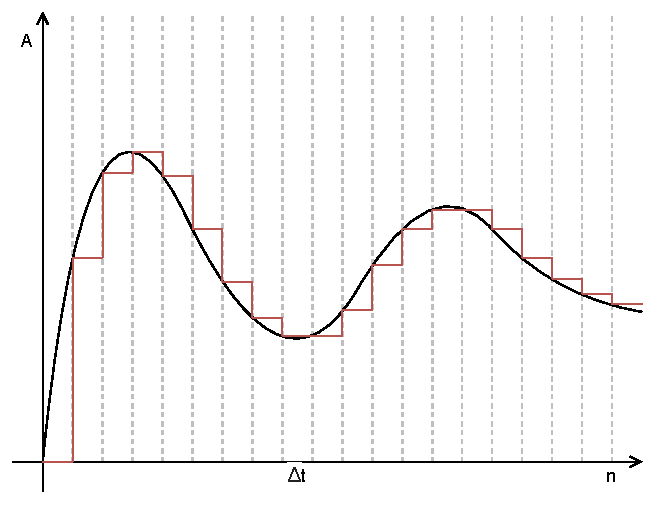
\includegraphics[width=0.5\textwidth]{includes/figures/defi_abtastrate.pdf}
    \end{center}
\end{bonus}

\begin{defi}{Sampling Rate}
    \begin{itemize}
        \item Wird zu selten abgetastet, erhalten wir eine sehr ungenaue Approximation des ursprünglichen analogen Signals

              \begin{center}
                  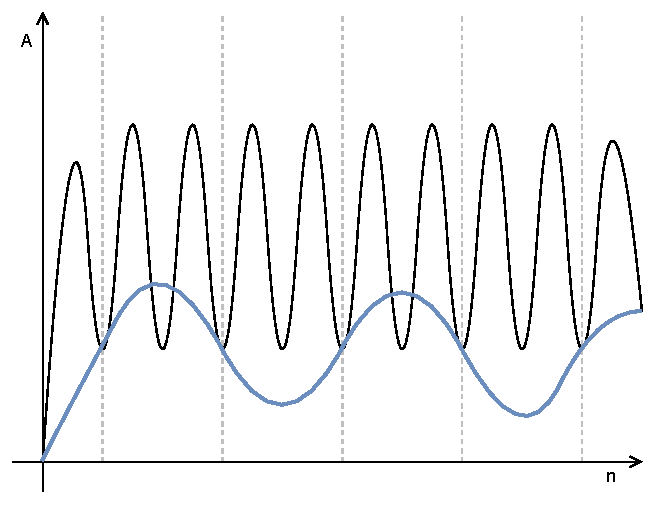
\includegraphics[width=0.5\textwidth]{includes/figures/defi_sampling_rate_error.pdf}
              \end{center}
        \item Wird zu häufig abgetastet, verbrachen wir Ressourcen, die eventuell für unseren Anwendungsfall nicht genutzt werden müssten
    \end{itemize}

    Nach den \emph{Nyquist-Shannon-Abtasttheorem} soll gelten: $\text{Abtastrate} > 2 \cdot \text{max. Frequenz}$

    Die Qualität des resultierenden Digitalsignals ist dabei abhängig von der Abtastrate und Auflösung.

    Die Bitrate ($\nicefrac{\text{bit}}{s}$) sei definiert als:
    \[
        \text{Bitrate} := \text{Kanäle} \cdot \text{Abtastrate (Hz)} \cdot \text{Auflösung (bit)}
    \]
\end{defi}

\begin{defi}{AD/DA-Wandlung}
    Zur Verarbeitung bzw. Erzeugung von analogen Signalen sind zwei Verarbeitungsprozesse notwendig.
    \begin{itemize}
        \item \emph{AD-Wandlung}: Analog $\to$ Digital
        \item \emph{DA-Wandlung}: Digital $\to$ Analog
    \end{itemize}

    Die technischen Vorrichtungen für die Umwandlung nennt man \emph{Wandler (engl. Converter)}.
    Das System für z. B. eine AD-Wandlung nennt man AD-Wandlung (\emph{Analog to Digital Converter (ADC)}).

    Wichtige Kenngrößen:
    \begin{itemize}
        \item \emph{Auflösung}: analoge Änderungen bei Änderung des Digitalwertes um $\pm 1$
        \item \emph{Digitaler Wertebereich} (in bits)
        \item \emph{Analoger Wertebereich} (z. B. in Volt)
        \item \emph{Geschwindigkeit}: Anzahl der Wandlungen pro Sekunde (ksps (kilo samples per second))
    \end{itemize}
\end{defi}

\begin{example}{AD/DA-Wandlung}
    \begin{center}
        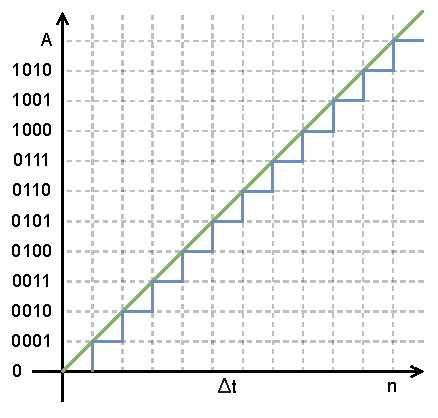
\includegraphics[width=0.33\textwidth]{includes/figures/example_ad_da.pdf}
    \end{center}

    Im optimalen Fall erhalten wir aus dem grünen analogen Signal das blaue digitale Signal.

    Dabei können u. a. folgende Fehler entstehen:

    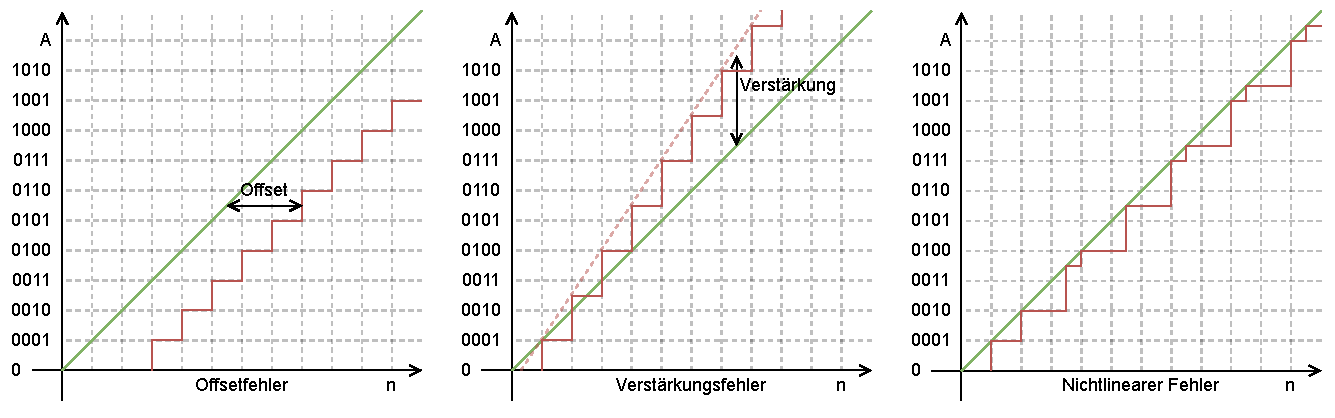
\includegraphics[width=\textwidth]{includes/figures/example_ad_da_error.pdf}
\end{example}

\begin{defi}{DA-Wandlung (Widerstandskette)}
    \emph{Direkt-Wandler} basieren auf einer Widerstandskette um $2^n$ mögliche Ausgangswerte zu realisieren.
    Hierzu benötigen wir $n$ Widerstände mit $k \ \Omega$.
    $n$ sei definiert als Anzahl der genutzten digitalen GPIO Pins $S_0 \to S_n$; in folgendem Beispiel sei $n = 2$.

    \begin{center}
        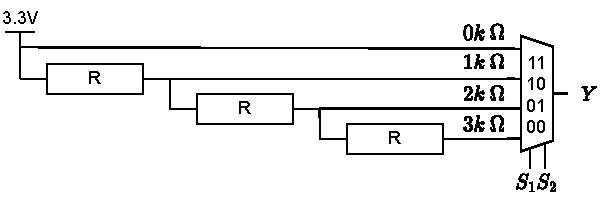
\includegraphics[width=0.5\textwidth]{includes/figures/defi_da_chain.pdf}
    \end{center}
\end{defi}

\begin{defi}{DA-Wandlung (Widerstandsnetzwerk)}
    Alternativ kann ein \emph{R-2R}-Widerstandsnetzwerk aushelfen:

    \begin{center}
        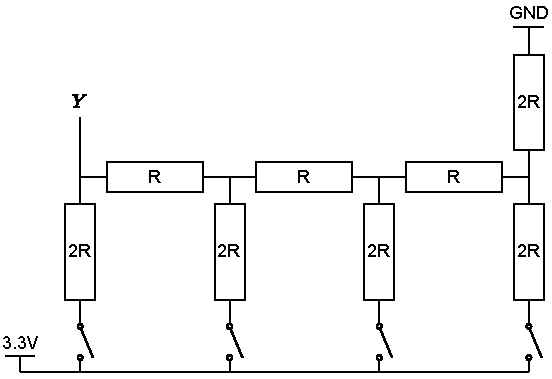
\includegraphics[width=0.5\textwidth]{includes/figures/defi_da_network.pdf}
    \end{center}
\end{defi}

\begin{defi}{AD-Wandlung (Inkrementalzähler)}
    Die Wandlung eines analogen Signals in eine Dualzahl ist technisch aufwändiger.

    Ein \emph{Inkrementalzähler} erstellt mit Hilfe einer Kombination aus Dualzähler und DA-Wandler aufsteigende Analogwerte.
    Mit einem Komperator wird der Vorgang unterbrochen, sobald der gemessene Analogwert erreicht wurde.

    \begin{center}
        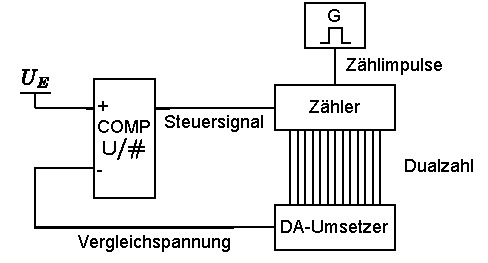
\includegraphics[width=0.5\textwidth]{includes/figures/defi_ad_inkrementalumsetzer.pdf}
    \end{center}
\end{defi}

\begin{defi}{AD-Wandlung (Flash Converter)}
    Alternativ kann man einen \emph{Flash Converter} nutzen:

    \begin{center}
        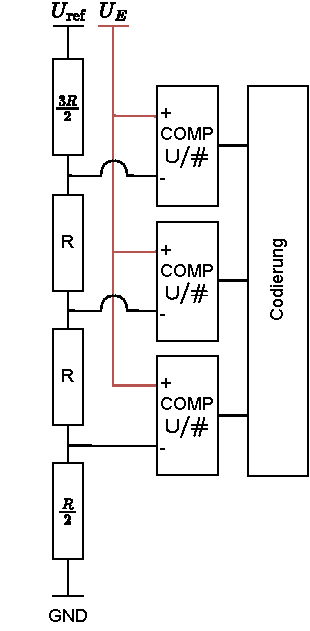
\includegraphics[width=0.25\textwidth]{includes/figures/defi_ad_flash_converter.pdf}
    \end{center}
\end{defi}

\begin{defi}{AD-Wandlung (Sigma Delta)}
    \emph{Sigma-Delta} AD-Wandler verfolgen eine ähnliche Idee wie die bisherigen Umsetzen, nur dass lediglich ein einzelnes Bit erzeugt wird.
    Der Wandler erzeugt dabei ein Bitstrom, dessen Mittelwert immer dem Eingangspegel entspricht.

    Dieser Vorgang geschieht i. d. R. mit einer hohen Frequenz (sog. Oversampling).

    Zur Umwandlung in einen Integer-Wert kann der Bitstrom für eine vorgegebene Zeit von Taktimpulsen betrachtet werden, und in dieser Zeit alle \texttt{HIGH}-Impulse gezählt wird.

    \begin{center}
        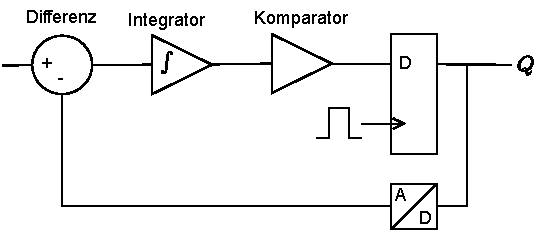
\includegraphics[width=0.5\textwidth]{includes/figures/defi_ad_sigma_delta.pdf}
    \end{center}
\end{defi}

\begin{bonus}{MSP432 Implementierung}
    Es stehen insgesamt 24 analoge Eingänge zur Verfügung.

    Neben dem \texttt{PxDIR} Register sind \texttt{PxSEL0} und \texttt{PxSEL1} auf \texttt{1} zu setzten.
\end{bonus}